\documentclass[../main.tex]{subfiles}
\begin{document}
\subsection{映射}
\begin{definition}
    设$X$和$Y$是集合,如果由$X$到$Y$的关系$f$同时满足:
    \begin{enumerate}
        \item $\mathrm{dom}f=X$;
        \item 对每一$X$的元素$x\in X$,\emph{有且只有一个}$Y$的元素$y\in Y$满足$\left(x,y\right)\in f$,
    \end{enumerate}
    则称$f$是由$X$到$Y$的\emph{映射(mapping)},记作$f:X\rightarrow Y$\footnote{记号$f:X\rightarrow Y$包含的信息是:
        \begin{enumerate}
            \item $X$、$Y$是集合;
            \item $f$是由$X$到$Y$的映射。
        \end{enumerate}
    }。对每一$\left(x,y\right)\in f$,称$y$是$x$在映射$f$下的\emph{值(value)},记作$f\left(x\right)$。
\end{definition}

\begin{figure}[htbp]
    \centering
    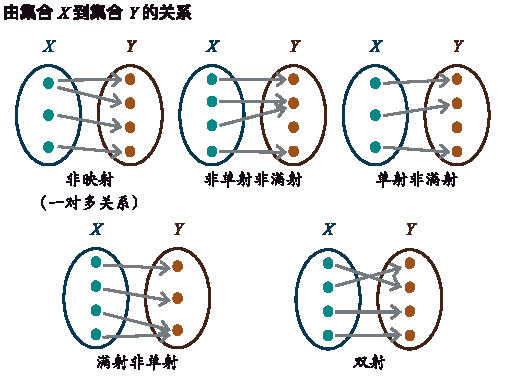
\includegraphics{../images/mapping.pdf}
    \caption{映射的定义}
    \label{fig:II.1.3}
\end{figure}

映射定义的第1条要求如果违反了,可通过对集合$X$的改动得到满足,而无需改动关系$f$本身。例如若$\mathrm{dom}f\subsetneqq X$,则令$X^\prime=\mathrm{dom}f$并改为讨论由$X^\prime$到$Y$的关系$f$,就可通过映射定义的第1条。然而映射定义的第2条,则图\ref{fig:II.1.3}中的第一个例子只是一个关系,而不是一个映射。

给定映射$f:X\rightarrow Y$,我们继续以下讨论:
\begin{itemize}
    \item 一般地,$Y$未必等于$\mathrm{ran}f$,集合$Y$称映射$f$的\emph{陪域(codomain)}。
    \item 若$\mathrm{ran}f=Y$则称映射$f$是\emph{满射(surjective mapping)}。图\ref{fig:II.1.3}中的第4和第5个例子都是满射。
    \item 若$A\subset X$,则集合$\left\{y|y\in Y\wedge\left(\forall x\in A,y=f\left(x\right)\right)\right\}$称集合$A$在映射$f$下的\emph{像(image)}。常见但易产生歧义的记法是$f\left(A\right)$。这一集合可用语言描述为:由集合$A$的所有元素在映射$f$下的值组成的集合。易证它是$Y$的子集。
    \item 若对任意$x_1,x_2\in X$,$f\left(x_1\right)=f\left(x_2\right)\Rightarrow x_1=x_2$,则称$f$是\emph{单射(injective mapping)}。可用语言描述为,“单射输出唯一地确定其输入”。图\ref{fig:II.1.3}中的第3和第5个例子都是满射。
\end{itemize}


(先补充数域的知识。)

我们在上节已了解过一个集合的元素可以与另一个集合的元素建立对应关系。本节我们主要关心的是满足某种规定的对应关系,称为映射,定义如下。

\begin{definition}[映射]
    从集合$X$到集合$Y$的映射(mapping)$f$,记为$f:X\rightarrow Y$,是$X$的所有元素与$Y$的部分或所有元素之间的对应关系,且每个$X$的元素只对应$Y$的一个元素。如果$y\in Y$是$x\in X$通过映射$f$的对应,则可写成$y=f\left(x\right)$,并称$f\left(x\right)$是$x$的像(image)。按上述定义,$x$只有一个像。$X$称为该映射$f$的定义域(domain),记为$\mathrm{dom}f$,$Y$称为该映射$f$的陪域(codomain)或到达域(target domain)。$x$的像$f\left(x\right)$是$Y$的子集,称为该映射$f$的值域(range),记为$\mathrm{ran}f$。
\end{definition}



当映射的陪域是实数集$\mathbb{R}^n$或复数集$\mathbb{C}^n$时,我们常常也称其为函数(function)。

\begin{definition}[映射的相等]
    若映射$f:X\rightarrow Y$和$g:X\rightarrow Y$满足$f\left(x\right)=g\left(x\right),\forall x\in X$,则这两个映射相等。
\end{definition}

\begin{definition}[恒等映射]
    恒等映射(identity mapping)$\mathrm{id}_A:A\rightarrow A$是由集合$A$到其自身的映射:$\mathrm{id}_A\left(a\right)=a,\forall a\in A$。
\end{definition}

\begin{figure}[htbp]
    \centering
    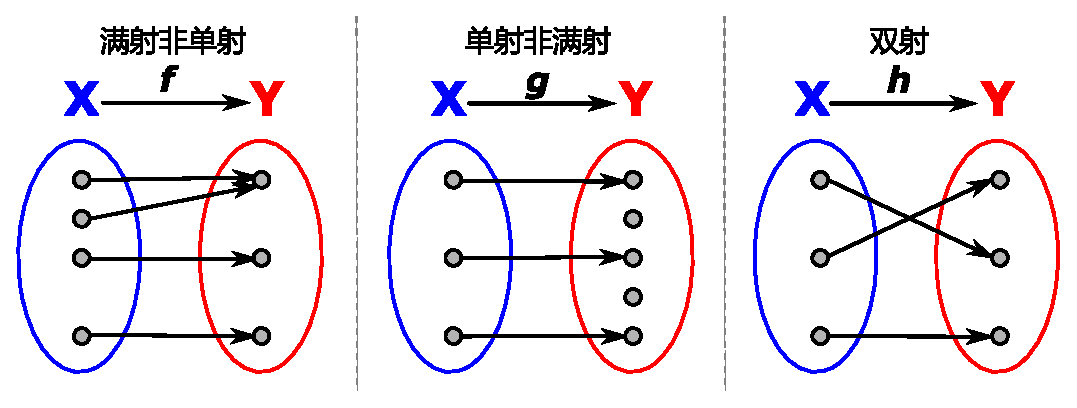
\includegraphics[width=0.5\textwidth]{../images/II.1.2.eps}
    \caption{满射、单射和双射}
    \label{fig:II.1.2}
\end{figure}

\begin{definition}[单射、双射、满射]
    对于映射$f:X\rightarrow Y$,若$f\left(x_1\right)=f\left(x_2\right)\Rightarrow x_1=x_2$,则映射$f$是单射(injective mapping)。若$\forall y\in Y\exists x\in X:f\left(x\right)=y$,则称$f$是满射(surjective mapping)。既是单射又是满射的映射叫双射(bijective mapping)。
\end{definition}

图\ref{fig:II.1.1}是一个非满射非单射的一般映射。图\ref{fig:II.1.2}给出的分而是满射非单射、单射非满射和双射的情况。

\begin{definition}[复合映射]
    设$f:X\rightarrow Y$和$g:Y\rightarrow Z$是两个映射。则$f$和$g$的复合映射(composite mapping),记为$g\circ f$,是从$X$到$Z$的映射:
    \[g\circ f\left(x\right)=g\left(f\left(x\right)\right),\forall x\in X\]
\end{definition}

\begin{theorem}
    对于映射$f:X\rightarrow Y$和$g: Y\rightarrow Z$,
    \begin{enumerate}
        \item 如果$f$和$g$都是满射,则$g\circ f$是满射
        \item 如果$g\circ f$是满射,则$g$是满射
        \item 如果$f$和$g$都是单射,则$g\circ f$是单射
        \item 如果$g\circ f$是单射,则$f$是单射
    \end{enumerate}
\end{theorem}
\begin{proof}
    “1”的证明:$g$是满射$\Leftrightarrow\forall z\in Z\exists y\in Y:g\left(y\right)=z$,$f$是满射$\Leftrightarrow\forall y\in Y\exists x\in X:f\left(x\right)=y$,所以$\forall z\in Z\exists x\in X:g\left(f\left(x\right)\right)=z$。

    “2”的证明:$g\circ f$是满射$\Leftrightarrow\forall z\in Z\exists x\in X:g\circ f\left(x\right)=z$,故对于$g$,$\forall z\in Z\exists y=f\left(x\right):g\left(y\right)=z$,即$g$是满射。

    “3”的证明:$g\left(f\left(x_1\right)\right)=g\left(f\left(x_2\right)\right)\Rightarrow f\left(x_1\right)=f\left(x_2\right)\Rightarrow x_1=x_2$。

    “4”的证明:$\because g\circ f$是单射,$\therefore g\left(f\left(x_1\right)\right)=g\left(f\left(x_2\right)\right)\Rightarrow x_1=x_2$。由映射的基本定义又有$f\left(x_1\right)=f\left(x_2\right)\Rightarrow g\left(f\left(x_1\right)\right)=g\left(f\left(x_2\right)\right)$。故$f\left(x_1\right)=f\left(x_2\right)\Rightarrow x_1=x_2$。
\end{proof}


\begin{definition}[逆映射]\label{def:II.1.14}
    对于映射$f:X\rightarrow Y$,如果存在一个映射$g:Y\rightarrow X$,使得复合映射$g\circ f$是恒等映射$\mathrm{id}_X$,则称映射$f$是可逆的(invertible),映射$g$是$f$的逆映射(inverse mapping)。
\end{definition}

关于逆映射,有一条重要的定理,使得在今后的数学陈述和推理中,我们可以默认——
\begin{theorem}\label{thm:II.1.7}
    双射必存在唯一逆映射。双射的逆映射也是双射。
\end{theorem}
\begin{proof}
    为了证明这一定理,我们首先证明一个引理:任一单射非满射均存在逆映射。

    设$f:X\rightarrow Y$是一个单射非满射,即$\exists y\notin\mathrm{ran}f,y\in Y$。由集合的相关定义此处必有$\left\{y|y\in\mathrm{ran}f\right\}\cup\left\{y|y\notin\mathrm{ran}f,y\in Y\right\}=Y$。

    现定义$g:Y\rightarrow X$,为使$g$为一个映射,它必须对$y\in\mathrm{ran}f$和$y\notin\mathrm{ran}f,y\in Y$均有定义。现将其定义为:
    \[
        g\left(y\right)=\left\{
        \begin{array}{ll}
            \left.x\right|_{f\left(x\right)=y}, & y\in\mathrm{ran}f           \\
            \text{任一}x\in X,                    & y\notin\mathrm{ran}f,y\in Y
        \end{array}
        \right.
    \]
    则有如下几条结论:
    \begin{enumerate}
        \item $g\left(y\right)$是映射。因为它对每一$y\in Y$均有定义且一个$y\in Y$只对应一个$x\in X$。
        \item $g$是满射。因为,仅$y\in\mathrm{ran}f$情况的定义式就已决定了$\mathrm{ran}g=X$。
        \item $g$是非单射。因为$g$是满射,再考虑$y\notin\mathrm{ran}f,y\in Y$情况的定义式,就可知$\exists x\in X$满足$x=g\left(y\right)=g\left(y^\prime\right)$,其中$y\neq y^\prime,y\in\mathrm{ran}f,y^\prime\notin\mathrm{ran}f,y^\prime\in Y$。
        \item $g$是$f$的逆映射。因为,对于任一$x\in X$均有$g\circ f\left(x\right)\equiv g\left(f\left(x\right)\right)=x$,即$g\circ f=\mathrm{id}_X$。
        \item 一般地,$g$是不唯一的。因为$y\notin\mathrm{f},y\in Y$的情况可定义$g\left(x\right)$等于任一$x\in X$,故只要集合$X$不是只有一个元素,那么$g$都不唯一。
    \end{enumerate}
    该引理证毕。

    现在正式证定理\ref{thm:II.1.7}。从上面定义的这个$g$继续,如果$g$是双射,则$g$不仅是满射,还是单射。由刚刚证完的引理,可用类似方法给$g$找一个逆映射$f^\prime:X\rightarrow Y$。而且,由于$\mathrm{ran}g\equiv X$,我们无需像定义$g$那样为$f^\prime$分出$x\notin\mathrm{ran}g,x\in X$的情况,因为不存在这种情况。故
    \[
        f^\prime\left(x\right)=\left.y\right|_{g\left(y\right)=x}
    \]
    是$g$的逆映射,且$f^\prime$是满射。而且,把$g$的定义代入上式有$f^\prime\left(x\right)=\left.y\right|_{g\left(y\right)=x}=\left.y\right|_{\left.x\right|_{f\left(x\right)=y}}=f\left(x\right)$,即$f^\prime$不是别的映射而恰为$f\left(x\right)$。即$g$的逆映射是唯一的。因$f^\prime$是满射故$f$是满射,而$f$本身就是单射,故$f$是双射。
\end{proof}
\end{document}